% Practice Test 03 — Oklahoma Edition
% Questions: 30 (21 MC + 9 SA)
% Generated by scripts/generate_practice_tests.py

\begin{practiceQuestion}{1-3-q29}{gsa}
\begin{questionText}
The graph shows a proportional relationship. Use the labeled point to find $k$, then determine $y$ when $x = 12$.

\begin{center}
\begin{tikzpicture}[scale=0.6]
  \draw[step=1,gray!20,thin] (0,0) grid (8,8);
  \draw[thick,->] (0,0) -- (8.5,0) node[right]{\small $x$};
  \draw[thick,->] (0,0) -- (0,8.5) node[above]{\small $y$};
  \foreach \x in {2,4,6,8} \draw (\x,0.07) -- (\x,-0.07) node[below]{\tiny \x};
  \foreach \y in {2,4,6,8} \draw (0.07,\y) -- (-0.07,\y) node[left]{\tiny \y};
  \draw[thick,funBlue] (0,0) -- (8,6);
  \fill[funBlue] (0,0) circle (2.5pt);
  \fill[funBlue] (4,3) circle (2.5pt) node[above left]{\small $(4, 3)$};
\end{tikzpicture}
\end{center}
\end{questionText}
\correctAnswer{$k = 0.75$; when $x = 12$, $y = 9$}
\explanation{$k = \frac{3}{4} = 0.75$. Then $y = 0.75 \times 12 = 9$.}
\end{practiceQuestion}

\begin{practiceQuestion}{1-6-q12}{mc}
\begin{questionText}
Store A sells $3$ notebooks for $\$7.50$. Store B sells $5$ notebooks for $\$11.25$. Which store offers the better deal?
\end{questionText}
\choiceA{Store A at $\$2.50$ each}
\choiceB{Store B at $\$2.25$ each}
\choiceC{Store A at $\$2.25$ each}
\choiceD{They cost the same}
\correctAnswer{B}
\explanation{Store A: $7.50 \div 3 = \$2.50$ each. Store B: $11.25 \div 5 = \$2.25$ each. Store B is cheaper.}
\end{practiceQuestion}

\begin{practiceQuestion}{1-7-q11}{mc}
\begin{questionText}
A model ship is $35$ cm long. The scale is $1 : 300$. What is the actual length of the ship?
\end{questionText}
\choiceA{$10.5$ m}
\choiceB{$105$ m}
\choiceC{$1{,}050$ m}
\choiceD{$35$ m}
\correctAnswer{B}
\explanation{Multiply: $35 \times 300 = 10{,}500$ cm $= 105$ m.}
\end{practiceQuestion}

\begin{practiceQuestion}{2-1-q25}{sa}
\begin{questionText}
A parking lot has spaces for $350$ cars. Currently $280$ spaces are filled. What percent of the lot is full?
\end{questionText}
\correctAnswer{$80\%$}
\explanation{Divide: $280 \div 350 = 0.80 = 80\%$.}
\end{practiceQuestion}

\begin{practiceQuestion}{2-4-q26}{gmc}
\begin{questionText}
The diagram shows the steps to find the final price of an item. What is the final price?

\begin{center}
\begin{tikzpicture}[scale=0.8, every node/.style={font=\small}]
  \node[draw,rounded corners,fill=funBlue!20,minimum width=2cm] (cost) at (0,0) {Cost: $\$40$};
  \node[draw,rounded corners,fill=funGreen!20,minimum width=2cm] (markup) at (4,0) {$+50\%$ markup};
  \node[draw,rounded corners,fill=funOrange!20,minimum width=2cm] (discount) at (8,0) {$-20\%$ discount};
  \node[draw,rounded corners,fill=funRed!20,minimum width=2cm] (tax) at (12,0) {$+10\%$ tax};
  \draw[thick,->] (cost) -- (markup);
  \draw[thick,->] (markup) -- (discount);
  \draw[thick,->] (discount) -- (tax);
\end{tikzpicture}
\end{center}
\end{questionText}
\choiceA{$\$48.00$}
\choiceB{$\$50.40$}
\choiceC{$\$52.80$}
\choiceD{$\$56.00$}
\correctAnswer{C}
\explanation{Markup: $40 \times 1.50 = \$60$. Discount: $60 \times 0.80 = \$48$. Tax: $48 \times 1.10 = \$52.80$.}
\end{practiceQuestion}

\begin{practiceQuestion}{2-7-q18}{mc}
\begin{questionText}
A package was estimated to weigh $10$ kg, but it actually weighs $12$ kg. A second package was estimated to weigh $50$ kg, but it actually weighs $52$ kg. Which estimate has the smaller percent error?
\end{questionText}
\choiceA{The first package}
\choiceB{The second package}
\choiceC{They have the same percent error}
\choiceD{Cannot be determined}
\correctAnswer{B}
\explanation{First: $\frac{2}{12} \times 100 \approx 16.7\%$. Second: $\frac{2}{52} \times 100 \approx 3.8\%$. The second has a smaller percent error.}
\end{practiceQuestion}

\begin{practiceQuestion}{2-8-q26}{gmc}
\begin{questionText}
The bar graph below compares the total cost of a $\$200$ purchase paid with a debit card vs.\ a credit card (at $18\%$ annual interest, paid after $1$ year). What is the difference in total cost?

\begin{center}
\begin{tikzpicture}[scale=0.7]
  \draw[thick,->] (0,0) -- (0,5.5) node[above] {Cost (\$)};
  \draw[thick,->] (0,0) -- (6,0);
  % Y axis labels
  \foreach \y/\label in {0/0, 1/50, 2/100, 3/150, 4/200, 5/250} {
    \draw (-0.1,\y) -- (0.1,\y);
    \node[left] at (-0.15,\y) {\footnotesize \$\label};
  }
  % Debit bar
  \fill[funBlue!70] (1,0) rectangle (2.5,4);
  \node[below] at (1.75,0) {\footnotesize Debit};
  \node[above] at (1.75,4) {\footnotesize \$200};
  % Credit bar
  \fill[funRed!70] (3.5,0) rectangle (5,4.72);
  \node[below] at (4.25,0) {\footnotesize Credit};
  \node[above] at (4.25,4.72) {\footnotesize \$236};
\end{tikzpicture}
\end{center}
\end{questionText}
\choiceA{$\$18$}
\choiceB{$\$36$}
\choiceC{$\$200$}
\choiceD{$\$236$}
\correctAnswer{B}
\explanation{Read the graph: $\$236 - \$200 = \$36$. The credit card costs $\$36$ more.}
\end{practiceQuestion}

\begin{practiceQuestion}{3-1-q19}{sa}
\begin{questionText}
What is the opposite of $-14$?
\end{questionText}
\correctAnswer{$14$}
\explanation{The opposite of $-14$ is $14$ because $-14 + 14 = 0$.}
\end{practiceQuestion}

\begin{practiceQuestion}{4-1-q12}{mc}
\begin{questionText}
Evaluate $\frac{3x + 1}{2}$ when $x = 5$.
\end{questionText}
\choiceA{$7$}
\choiceB{$8$}
\choiceC{$8.5$}
\choiceD{$7.5$}
\correctAnswer{B}
\explanation{Substitute: $\frac{3(5) + 1}{2} = \frac{15 + 1}{2} = \frac{16}{2} = 8$.}
\end{practiceQuestion}

\begin{practiceQuestion}{4-2-q11}{mc}
\begin{questionText}
How many terms are in the simplified form of $8b - 3 + 2b + 5 - b$?
\end{questionText}
\choiceA{$5$}
\choiceB{$3$}
\choiceC{$2$}
\choiceD{$1$}
\correctAnswer{C}
\explanation{Combine variable terms: $8b + 2b - b = 9b$. Combine constants: $-3 + 5 = 2$. Simplified: $9b + 2$, which has $2$ terms.}
\end{practiceQuestion}

\begin{practiceQuestion}{5-3-q16}{mc}
\begin{questionText}
Solve $8(x + 1) = 48$.
\end{questionText}
\choiceA{$x = 5$}
\choiceB{$x = 6$}
\choiceC{$x = 7$}
\choiceD{$x = \dfrac{47}{8}$}
\correctAnswer{A}
\explanation{Divide by $8$: $x + 1 = 6$. Subtract $1$: $x = 5$. Check: $8(5 + 1) = 8(6) = 48$ \checkmark.}
\end{practiceQuestion}

\begin{practiceQuestion}{5-4-q13}{mc}
\begin{questionText}
A shirt is on sale for $\dfrac{2}{3}$ of its original price. After using a $\$5$ coupon, you pay $\$15$. What equation finds the original price $p$?
\end{questionText}
\choiceA{$\dfrac{2}{3}p + 5 = 15$}
\choiceB{$p - \dfrac{2}{3} - 5 = 15$}
\choiceC{$\dfrac{2}{3}p - 5 = 15$}
\choiceD{$\dfrac{2}{3}(p - 5) = 15$}
\correctAnswer{C}
\explanation{Sale price is $\frac{2}{3}p$. After the $\$5$ coupon: $\frac{2}{3}p - 5 = 15$.}
\end{practiceQuestion}

\begin{practiceQuestion}{5-5-q02}{mc}
\begin{questionText}
Solve $-3n + 6 \leq 0$.
\end{questionText}
\choiceA{$n \leq 2$}
\choiceB{$n \leq -2$}
\choiceC{$n \geq 2$}
\choiceD{$n \geq -2$}
\correctAnswer{C}
\explanation{Subtract $6$: $-3n \leq -6$. Divide by $-3$ and flip the sign: $n \geq 2$.}
\end{practiceQuestion}

\begin{practiceQuestion}{5-6-q05}{mc}
\begin{questionText}
Which inequality is shown by a closed circle at $7$ with shading to the left?
\end{questionText}
\choiceA{$x > 7$}
\choiceB{$x < 7$}
\choiceC{$x \geq 7$}
\choiceD{$x \leq 7$}
\correctAnswer{D}
\explanation{Closed circle means the endpoint is included, shading left means less than or equal to: $x \leq 7$.}
\end{practiceQuestion}

\begin{practiceQuestion}{6-2-q27}{gmc}
\begin{questionText}
The two rectangles below represent the same room drawn at two different scales. The original uses $1$ cm $= 6$ m. What scale does the new drawing use?

\begin{center}
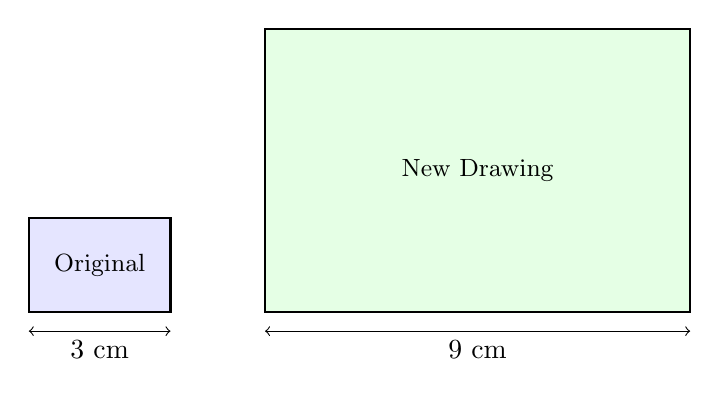
\begin{tikzpicture}[scale=0.6]
  % Original
  \draw[thick,fill=blue!10] (0,0) rectangle (3,2);
  \node at (1.5,1) {\small Original};
  \draw[<->] (0,-0.4) -- (3,-0.4);
  \node[below] at (1.5,-0.4) {$3$ cm};
  % New
  \draw[thick,fill=green!10] (5,0) rectangle (14,6);
  \node at (9.5,3) {\small New Drawing};
  \draw[<->] (5,-0.4) -- (14,-0.4);
  \node[below] at (9.5,-0.4) {$9$ cm};
\end{tikzpicture}
\end{center}
\end{questionText}
\choiceA{$1$ cm $= 2$ m}
\choiceB{$1$ cm $= 3$ m}
\choiceC{$1$ cm $= 6$ m}
\choiceD{$1$ cm $= 18$ m}
\correctAnswer{A}
\explanation{Scale ratio: $9 \div 3 = 3$. The new drawing is $3$ times bigger. Actual length: $3 \times 6 = 18$ m. New scale: $18 \div 9 = 2$ m per cm.}
\end{practiceQuestion}

\begin{practiceQuestion}{6-3-q20}{sa}
\begin{questionText}
A triangle has two sides of length $8$ cm and $12$ cm. What is the range of possible lengths for the third side?
\end{questionText}
\correctAnswer{Greater than $4$ cm and less than $20$ cm}
\explanation{By the triangle inequality: $12 - 8 < \text{third side} < 12 + 8$, so $4 < \text{third side} < 20$.}
\end{practiceQuestion}

\begin{practiceQuestion}{6-4-q25}{sa}
\begin{questionText}
A triangle has angles $60°$, $60°$, and $60°$, and one side measures $10$ cm. How many triangles can be drawn?
\end{questionText}
\correctAnswer{Exactly one}
\explanation{AAA alone gives many, but specifying a side length fixes the size. A triangle with all $60°$ angles is equilateral, so all sides are $10$ cm. Exactly one triangle.}
\end{practiceQuestion}

\begin{practiceQuestion}{6-5-q01}{mc}
\begin{questionText}
You slice a rectangular prism with a cut parallel to its base. What shape is the cross-section?
\end{questionText}
\choiceA{Triangle}
\choiceB{Circle}
\choiceC{Rectangle}
\choiceD{Pentagon}
\correctAnswer{C}
\explanation{A horizontal cut parallel to the base of a rectangular prism produces a rectangle the same shape as the base.}
\end{practiceQuestion}

\begin{practiceQuestion}{6-6-q05}{mc}
\begin{questionText}
Two complementary angles are $(x + 15)°$ and $(2x)°$. Find the smaller angle.
\end{questionText}
\choiceA{$25°$}
\choiceB{$40°$}
\choiceC{$50°$}
\choiceD{$65°$}
\correctAnswer{B}
\explanation{$x + 15 + 2x = 90$. Combine: $3x + 15 = 90$. Solve: $3x = 75$, $x = 25$. Angles: $25 + 15 = 40°$ and $2(25) = 50°$. The smaller is $40°$.}
\end{practiceQuestion}

\begin{practiceQuestion}{7-4-q06}{mc}
\begin{questionText}
An L-shaped room can be split into a $10$ ft by $8$ ft rectangle and a $4$ ft by $6$ ft rectangle. What is the total floor area?
\end{questionText}
\choiceA{$56$ ft$^2$}
\choiceB{$80$ ft$^2$}
\choiceC{$104$ ft$^2$}
\choiceD{$128$ ft$^2$}
\correctAnswer{C}
\explanation{$10 \times 8 = 80$ ft$^2$. $4 \times 6 = 24$ ft$^2$. Total: $80 + 24 = 104$ ft$^2$.}
\end{practiceQuestion}

\begin{practiceQuestion}{7-5-q30}{gsa}
\begin{questionText}
A box without a lid is shown below. What is the total surface area (including the bottom but NOT the top)?

\begin{center}
\begin{tikzpicture}[scale=0.4]
  % Front face
  \draw[thick,funBlue,fill=funBlue!10] (0,0) -- (8,0) -- (8,5) -- (0,5) -- cycle;
  % Top (open — dashed)
  \draw[thick,dashed,gray] (0,5) -- (3,7) -- (11,7) -- (8,5);
  % Right face
  \draw[thick,funBlue,fill=funBlue!15] (8,0) -- (11,2) -- (11,7) -- (8,5) -- cycle;
  % Labels
  \draw[thick,funRed,<->] (0,-0.7) -- (8,-0.7);
  \node[below,funRed] at (4,-0.7) {$8$ cm};
  \draw[thick,funRed,<->] (11.5,2) -- (11.5,7);
  \node[right,funRed] at (11.5,4.5) {$5$ cm};
  \draw[thick,funRed,<->] (8,-0.7) -- (11,-0.7+2);
  \node[below right,funRed] at (9.5,0) {$3$ cm};
\end{tikzpicture}
\end{center}
\end{questionText}
\correctAnswer{$134$ cm$^2$}
\explanation{Bottom: $8 \times 3 = 24$ cm$^2$. Front and Back: $2(8 \times 5) = 80$ cm$^2$. Two sides: $2(3 \times 5) = 30$ cm$^2$. Total (no top): $24 + 80 + 30 = 134$ cm$^2$.}
\end{practiceQuestion}

\begin{practiceQuestion}{7-6-q14}{mc}
\begin{questionText}
A rectangular prism is $8$ in by $5$ in by $4$ in. Another is $10$ in by $4$ in by $4$ in. Which has more volume and by how much?
\end{questionText}
\choiceA{First prism, by $10$ in$^3$}
\choiceB{Second prism, by $10$ in$^3$}
\choiceC{First prism, by $20$ in$^3$}
\choiceD{They have the same volume}
\correctAnswer{D}
\explanation{First: $8 \times 5 \times 4 = 160$ in$^3$. Second: $10 \times 4 \times 4 = 160$ in$^3$. They have the same volume.}
\end{practiceQuestion}

\begin{practiceQuestion}{8-1-q02}{mc}
\begin{questionText}
A researcher wants to know the average height of seventh graders in a state. She measures the heights of $100$ seventh graders from different schools. What is the sample?
\end{questionText}
\choiceA{All seventh graders in the state}
\choiceB{All students in the schools she visited}
\choiceC{The $100$ seventh graders she measured}
\choiceD{The tallest seventh graders}
\correctAnswer{C}
\explanation{The sample is the smaller group chosen from the population — the $100$ students measured.}
\end{practiceQuestion}

\begin{practiceQuestion}{8-3-q24}{sa}
\begin{questionText}
Class A: median $90$, IQR $6$. Class B: median $83$, IQR $14$. Which class is more consistent?
\end{questionText}
\correctAnswer{Class A}
\explanation{Class A has a smaller IQR ($6$ vs.\ $14$), meaning the middle $50\%$ of scores are more tightly clustered.}
\end{practiceQuestion}

\begin{practiceQuestion}{8-4-q19}{sa}
\begin{questionText}
Data: $30, 35, 40, 45, 50$. Find the mean and range.
\end{questionText}
\correctAnswer{Mean $= 40$; Range $= 20$}
\explanation{Mean: $\frac{30+35+40+45+50}{5} = \frac{200}{5} = 40$. Range: $50 - 30 = 20$.}
\end{practiceQuestion}

\begin{practiceQuestion}{8-5-q04}{mc}
\begin{questionText}
Data: $12, 15, 21, 23, 27, 30, 35$. In a stem-and-leaf plot, what are the stems?
\end{questionText}
\choiceA{$1, 2, 3$}
\choiceB{$2, 5, 1, 3, 7, 0, 5$}
\choiceC{$12, 15, 21, 23, 27, 30, 35$}
\choiceD{$10, 20, 30$}
\correctAnswer{A}
\explanation{The stems are the tens digits: $1$ (for $12, 15$), $2$ (for $21, 23, 27$), $3$ (for $30, 35$).}
\end{practiceQuestion}

\begin{practiceQuestion}{8-7-q13}{mc}
\begin{questionText}
A line graph shows a company's profits: Q1 $\$50{,}000$, Q2 $\$60{,}000$, Q3 $\$55{,}000$, Q4 $\$70{,}000$. What was the increase from Q1 to Q4?
\end{questionText}
\choiceA{$\$10{,}000$}
\choiceB{$\$15{,}000$}
\choiceC{$\$20{,}000$}
\choiceD{$\$70{,}000$}
\correctAnswer{C}
\explanation{$\$70{,}000 - \$50{,}000 = \$20{,}000$.}
\end{practiceQuestion}

\begin{practiceQuestion}{9-4-q27}{gmc}
\begin{questionText}
The table shows a probability model for a spinner. The spinner is spun $100$ times and the results are shown. Does the observed data support the model?

\begin{center}
\begin{tabular}{|c|c|c|}
\hline
\textbf{Color} & \textbf{Model $P$} & \textbf{Observed Frequency} \\
\hline
Red & $0.40$ & $38$ \\
\hline
Blue & $0.35$ & $36$ \\
\hline
Yellow & $0.25$ & $26$ \\
\hline
\end{tabular}
\end{center}
\end{questionText}
\choiceA{No, the data is very different from the model}
\choiceB{Yes, the observed frequencies are close to the predicted values}
\choiceC{No, because Red appeared fewer times than predicted}
\choiceD{The model cannot be checked with only $100$ spins}
\correctAnswer{B}
\explanation{Predicted: Red $= 40$, Blue $= 35$, Yellow $= 25$. Observed: $38$, $36$, $26$. These are close, supporting the model.}
\end{practiceQuestion}

\begin{practiceQuestion}{9-6-q01}{mc}
\begin{questionText}
What is the probability of flipping two coins and getting heads on both?
\end{questionText}
\choiceA{$\frac{1}{2}$}
\choiceB{$\frac{1}{3}$}
\choiceC{$\frac{1}{4}$}
\choiceD{$\frac{3}{4}$}
\correctAnswer{C}
\explanation{Sample space: HH, HT, TH, TT ($4$ outcomes). Only HH is heads-heads. $P = \frac{1}{4}$.}
\end{practiceQuestion}

\begin{practiceQuestion}{9-7-q20}{sa}
\begin{questionText}
You roll a die $90$ times to simulate a $\frac{1}{6}$ probability event. How many times do you expect the event to occur?
\end{questionText}
\correctAnswer{$15$}
\explanation{$90 \times \frac{1}{6} = 15$.}
\end{practiceQuestion}
